% Chapter Template

\chapter{Synrad3D} % Main chapter title

\label{soft} % Change X to a consecutive number; for referencing this chapter elsewhere, use \ref{ChapterX}

\lhead{Chapter 4. \emph{Synrad3D}} % Change X to a consecutive number; this is for the header on each page - perhaps a shortened title



%----------------------------------------------------------------------------------------
%	SECTION 2
%----------------------------------------------------------------------------------------

\section{Introduction to Synrad3D}
\label{Synrad3d}
\srthree is a program built in Bmad. It was written by David Sagan using a photon scattering model developed by Gerry Dugan, both of them from Cornell University. 
 
\srthree  simulates the production and scattering of synchrotron radiation generated by an electron beam in a high energy machine. \citep{syn}. The \srthree program uses the Monte Carlo method for photon generation, scattering, and absorption calculations.
\subsection{Physics of Synrad3D}


This section is based on the Synrad3D user manual\cite{syn} 

To generate photons, a section of the machine is selected.  The user sets the total number of photons to be generated. \srthree calculates how many photons need to be generated within each machine element. The local bending field at the beam orbit is used to determine the photon spectrum.

Each photon is tracked from the point of origin to the point at which it hits the vacuum chamber wall. The angle of incidence relative to the local normal to the vacuum chamber is computed. The scattering probability is calculated, using this angle and the photon's energy. Using the value of this probability, the photon is either absorbed at this location, or scattered. If it is scattered, the scattering is taken to be elastic. That is, photon energy does not change. This ignores any florescence. Surface roughness, on the other hand is taken into account so there is a diffuse component to the scattering. Then the photon is tracked to the next hit on the vacuum chamber wall, and the probability of scattering is again computed. This process goes on until the photon is absorbed.
\subsubsection{Photon Generation}
Photon generation is based on the standard synchrotron radiation formulas, applicable for dipoles and quadrupoles. The radiation is assumed to be incoherent.

\texttt{Synrad3D}\xspace  slices up each element longitudinally and generates photons from each slice. The number of photons generated in a slice weighted by the local probability of photon emission which depends on the local orbit curvature.

Photon generation is based upon the local field along the beam orbit. Thus, for example, particles in a bending magnet will radiate. The beam orbit is calculated from such things as the settings of steering elements, element misalignments, etc. as given in the lattice file. The beam orbit is the closed orbit. 

When a photon is generated at a given longitudinal position, the beam's emittances and centroid are used so that the resulting photon distribution mirrors the Gaussian positional distribution of the beam. Horizontal/vertical coupling is taken into account in this calculation. The photon energy distribution will be the standard energy spectrum of photons generated in a bend.

A photon's initial angular orientation is generated by first using a random number generator to generate an angular orientation using a probability function that corresponds to the beam's angular distribution. The generated photons will have the proper correlation between photon energy and photon angle. The plane of the bend may not be horizontal.
\subsubsection{Photon Scattering} 

  \begin{figure}
  \centering
  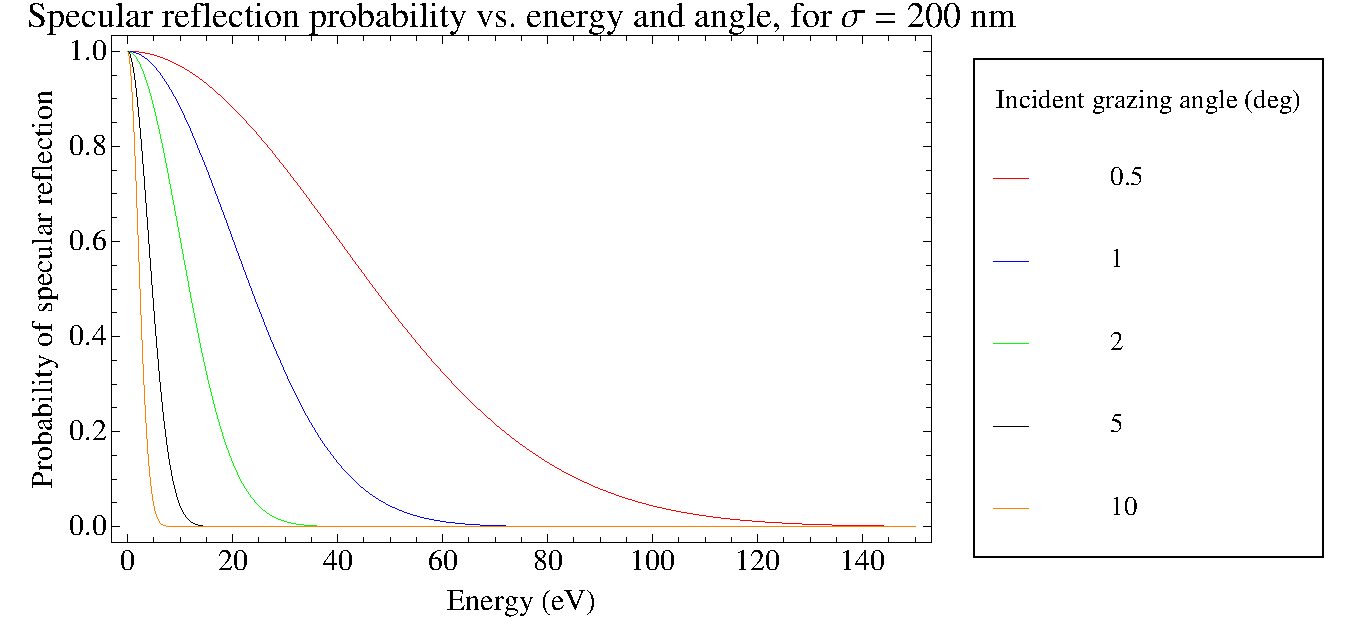
\includegraphics[width=6in]{Synrad3d/specular-probability.pdf}
  \caption[Specular reflection probability vs. photon energy and angle]
{\label{f:spec.prob}
Specular reflection probability~\cite{b:beckmann}, vs. photon energy
and angle, for an rms surface roughness of 200 nm.}
%\footnotesize{Picture taken from \citep{syn}}
  \end{figure}
   

The probability that a photon will reflect specularly from a surface depends on the the rms surface roughness $\sigma$, the wavelength of the photon $\lambda$, and the grazing angle. As shown in equation \ref{eq:SpRe}:
the formula for this probability is~\cite{b:beckmann}
   \begin{equation}
   \label{eq:SpRe}
P_{\textrm{spec}}=\textrm{e}^{-g(x,y)},
\end{equation}
where
   \begin{equation}
g(x,y)=\frac{4\pi^{2}\sigma^{2}(x+y)^{2}}{\lambda^{2}}
  \end{equation}
where $x$ is the cosine of the incident polar angle, and $y$ is the
cosine of the scattered polar angle.

For a typical technical vacuum chamber surface, the rms surface roughness $\sigma \gtrsim 200$ nm is
greater than most of the X-ray wavelengths of interest. In this regime diffuse scattering from the surface dominates over specular reflection. This is illustrated in Fig.~\ref{f:spec.prob}.
The model for diffuse scattering used by \srthree assumes a Gaussian distribution for both the surface height variations (rms $\sigma$) and for the transverse distribution.

The most general expression for the diffusely scattered power is complex, and involves an infinite sum.  However, the expression simplifies substantially in the limit $g(x,y)\gg 1.$ For very rough surfaces corresponding to technical vacuum chambers, for which typically $\sigma \gg \lambda$, this condition is satisfied over much of the region of interest.

\subsection{Input Files}
The input files used by \srthree are the following:
\subsubsection*{Synrad3D Main Input File (SMIF)}
\label{smif}
This file should be specified on the command line that invokes synrad3d, if it is not specified, it will select the default name "synrad3d.init". This file contains the parameters of the simulation
\begin{itemize}
\item The region where radiation is produced specified by the index numbers of elements in the lattice.
\item The direction in which the photons are travelling when initially created. 
\item The minimun number of photons that need to be generated before \srthree will stop the simulation.  
\item the number of photons generated throughout the radiation production region.
\item The minimun distance to track the particle beam between emission points.
\item The particle beam size.
\item The lattice file defining the optics of the accelerator.
\item The wall file defining the vacuum chamber's geometry.
\item The name of the output file.
\item The surface roughness for the default surface.
\item The surface roughness correlation for the default surface.
\item The surface reflection file for non-default surface.
\item The minimun and maximun initial energy values to be filtered by \srthree .
\end{itemize}
There are other parameters that can be specified in the SMIF, but are not mentioned here, because they are not relevant to this work.

\subsubsection*{Lattice File}
This file cointains the complete description of the elements of the lattice, defining the optics of the machine. This file must be specified in the SMIF.
\subsubsection*{Vacuum Chamber Wall Definition file}
The file specified in the SMIF defines the cross section of the vacuum chamber's wall at a number of longitudinal positions.
\subsubsection*{Chamber Surface Reflectivity file}
The reflectivity of the vacuum chamber wall can be described on the surface reflection file specified in the SMIF. If no file is specified \srthree will use the default reflectivity, which  is based on the refletivity of a Carbon film on Aluminum substrate. 

\subsection{Output Files}

\subsubsection*{Synrad3d Main Output File}
The name of this file must be specified in the SMIF. This file contains the information from the SMIF and the data generated for each photon. This information consists of:
\begin{itemize}
\item The number of the photon.
\item The number of times the photon hit the wall.
\item The photon energy.
\item The position where the photon was generated.
\item The position where the photon was absorbed.
\item The distance traveled by the photon.
\item The type of the lattice element where the photon was absorbed.
\end{itemize}

%----------------------------------------------------------------------------------------
%	SECTION 1
%----------------------------------------------------------------------------------------



%--------------------------------------------------------------------------------------------
\section{Tools}
Given the nature of routines described in \ref{Synrad3d}, using enough photons to obtain statistically valid results, running this program would take months in a regular commercial computer. To surpass this limitation the CERN {\it Lxplus} computing cluster was employed.
\subsection{Lxplus}
\label{lxplus}
The Lx Public Login Service or Lxplus is a login service offered to all CERN users. This cluster consists in several public machines running SLC5 in 64 bit mode, where all interactive and batch systems are built on top of the CERN standart Unix Enviroment. There is a wide range of shells available, that can be sorted in two groups: the C-shell like and the Bourne-shell like. We used Bash because of the full Linux based facilities. Since this machines are not to be used to store data a Workspace was made in the AFS file system that is accesible through normal system commands. Running CPU intense jobs in those machines is prohibited, so a system of jobs submissions to a set of queues with different limits on the available resources is at the disposal of the Lxplus user.
